%=================================
\begin{name}
	{\tenchude}
	{\tendethi}
	{\tentruong}
	{\thoigian}
\end{name}
\Opensolutionfile{ans}[ans/ansVN-1]
%%==========Câu 1
\begin{ex}%[2D1Y1-1]
	Cho hàm số $y=\dfrac{x-1}{x+2}$. Mệnh đề nào sau đây là mệnh đề đúng?
	\choice
	{Hàm số đồng biến trên $\mathbb{R} \setminus \left\lbrace -2\right\rbrace $}
	{\True Hàm số đồng biến trên từng khoảng xác định}
	{Hàm số đồng biến trên $\mathbb{R}$}
	{Hàm số nghịch biến trên từng khoảng xác định}
	\loigiai{
		\begin{itemize}
			\item [$\bullet$] Ta có $y'=\dfrac{3}{\left(x+2 \right) ^2}>0$, $\forall x \ne -2$.
			\item [$\bullet$] Vậy hàm số đồng biến trên từng khoảng xác định.
		\end{itemize}
	}
\end{ex}

%%==========Câu 2
\begin{ex}%[2D1Y2-2]
	Cho hàm số $ y=f(x)$ có bảng biến thiên như hình vẽ sau
	\begin{center}
		
\begin{tikzpicture}[>=stealth]
			\tkzTabInit[nocadre=false,lgt=1.2,espcl=2,deltacl=0.5]{$x $ /.6, $ f'(x)$ /.6, $ f(x)$ /2}
			{$-\infty $, $ 0 $, $ 3 $, $+\infty$}
			\tkzTabLine{,+, $ 0 $,-, $ 0 $,+, }
			\tkzTabVar{-/ $-\infty $,+/ $ 2 $,-/ $-4 $,+/ $+\infty$}
		\end{tikzpicture}
	\end{center} 
	Hàm số đã cho đạt cực tiểu tại điểm nào sau đây?
	\choice
	{$x=2$}
	{\True $ x=3$}
	{$x=0$}
	{$x=-4$}
	\loigiai{
		Từ bảng biến thiên, hàm số đã cho đạt cực tiểu tại điểm $ x=3 $ với $ y=-4 $.
	}
\end{ex}

%%==========Câu 3
\begin{ex}%[2D1Y3-1]
	Cho hàm số $y=f\left( x \right)$ liên tục trên $\left[-3;2\right]$ và có bảng biến thiên như hình bên.
	\begin{center}
		
\begin{tikzpicture}
			\tkzTabInit[nocadre=false,lgt=1.2,espcl=1.6]
			{$x$ /0.6,$y'$ /0.6,$y$ /2}
			{$-3$,$-1$,$0$,$1$,$2$}
			\tkzTabLine{,+,$0$,-,$0$,+,$0$,-,}
			\tkzTabVar{-/$-2$, +/$3$,-/$0$,+/$2$,-/$1$}
		\end{tikzpicture}
	\end{center} 
	Gọi $M$, $m$ lần lượt là giá trị lớn nhất và giá trị nhỏ nhất của hàm số $y=f\left( x \right)$ trên đoạn $\left[-1;2\right]$. Tính $M+m$.
	\choice
	{$1$}
	{$2$}
	{\True $3$}
	{$4$}
	\loigiai{
		\begin{itemize}
			\item [$\bullet$] Quan sát bảng biến thiên ta thấy trên đoạn $\left[-1;2\right]$ thì hàm số đạt $GTNN$ bằng $0$ tại $ x=0$ và đạt $GTLN$ bằng $3$ tại $ x=-1$.
			\item [$\bullet$] Do đó $M=3$ và $m=0$. Suy ra $M+m=3+0=3$.
		\end{itemize}
	}
\end{ex}

%%==========Câu 4
\begin{ex}%[2D1Y4-1]
	Đồ thị của hàm số $ y=\dfrac{2x-3}{x-1}$ có đường tiệm cận ngang là đường thẳng
	\choice
	{$x=1$}
	{\True $y=2$}
	{$x=2$}
	{$y=1$}
	\loigiai
	{
		\begin{itemize}
			\item [$\bullet$] 	Ghi nhớ: Đồ thị hàm số $y=\dfrac{ax+b}{cx+d}$ có đường tiệm cận ngang là $y=\dfrac{a}{c}$.
			\item [$\bullet$] Áp dụng, ta được $y=2$ là đường tiệm cận ngang.
		\end{itemize}
		
	}
\end{ex}

%%==========Câu 5
\begin{ex}%[2D1B5-4]
	Số giao điểm của đồ thị hàm số $ y=x^3-x^2 $ và đồ thị hàm số $ y=-x^2+5x $ là
	\choice
	{$1$}
	{$2$}
	{$0$}
	{\True $ 3$}
	\loigiai{
		Phương trình hoành độ giao điểm của hai đồ thị là
		\[x^3-x^2=-x^2+5x\Leftrightarrow x^3-5x=0\Leftrightarrow\hoac{&x=0\\&x=\sqrt{5}\\&x=-\sqrt{5}.}\]
	}
\end{ex}

%%==========Câu 6
\begin{ex}%[2D1Y5-1]
	\immini[thm]{
		Đồ thị hình bên là của một trong bốn hàm số sau đây. Hỏi đó là hàm số nào?
		\choice
		{$y=x^4-2x^2+1$}
		{$y=x^4-2x^2$}
		{$y=-x^4+2x^2+1$}
		{\True $y=-x^4+2x^2$}
	}{
		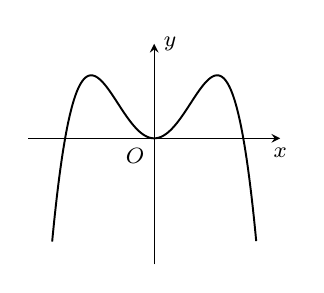
\begin{tikzpicture}[smooth,samples=300,scale=0.8,>=stealth,font=\footnotesize]
			\draw[->] (-2,0)--(2,0) node[below]{$x$};
			\draw[->] (0,-2)--(0,1.5) node[right]{$y$};
			\draw (0,0) node[below left]{$O$};
			\draw[line width=0.7pt,domain=-1.62:1.62] plot(\x,{-(\x)^4+2*(\x)^2});
	\end{tikzpicture}}
	\loigiai{
		Đồ thị trên là của hàm số dạng $y=ax^4+bx^2+c$ với $a<0$.\\
		Vì đồ thị đi qua điểm $O(0;0)$ nên hàm số cần tìm là $y=-x^4+2x^2$.
	}
\end{ex}

%%==========Câu 7
\begin{ex}%[2D1B5-4]
	Cho hàm số $y=x^3-3x$ có đồ thị $(C)$. Tìm số giao điểm của $(C)$ và trục hoành.
	\choice
	{$ 2$}
	{\True $ 3$}
	{$ 0$}
	{$ 1$}
	\loigiai{
		Xét phương trình hoành độ giao điểm
		$$x^3-3x=0\Leftrightarrow \hoac{& x=0 \\ & x=\pm \sqrt{3}.}$$
		Vậy $(C)$ và trục hoành có $3$ điểm chung.
	}
\end{ex}

%%==========Câu 8
\begin{ex}%[2D1Y5-6]
	Hệ số góc $k$ của tiếp tuyến đồ thị hàm số $y=x^3+1$ tại điểm $M\left(1;2\right)$ là
	\choice
	{$k=5$}
	{\True $k=3$}
	{$k=4$}
	{$k=12$}
	\loigiai{
		Ta có $y'=3x^2\Rightarrow$ hệ số góc của tiếp tuyến của đồ thị hàm số tại điểm $M$ là $k=y'(1)=3$.
	}
\end{ex}


%%==========Câu 9
\begin{ex}%[2D1B5-3]
	\immini[thm]{Cho hàm số $y=f(x)$ có bảng biến thiên như hình bên. Số nghiệm thực của phương trình $2f(x)-3=0$ là
		\choice
		{$1$}
		{$4$}
		{$2$}
		{\True $0$}}{
		
\begin{tikzpicture}
			\tikzset{double style/.append style = {draw=\tkzTabDefaultWritingColor,double=\tkzTabDefaultBackgroundColor,double distance=2pt}}
			\tkzTabInit[nocadre=false,lgt=1,espcl=1.3,deltacl=0.6] %phần bắt buộc
			{$x$/0.6, $y'$/0.6, $y$/2.2} %phần bắt buộc
			{$-\infty$, $-3$, $-2$, $-1$, $+\infty$} % hàng 1 cột 2
			\tkzTabLine{,+,z,-,d,-,z,+,}
			\tkzTabVar{-/$-\infty$,+/$0$,-D+/$-\infty$/$+\infty$,-/$2$,+/$+\infty$}
	\end{tikzpicture}}
	\loigiai
	{
		Phương trình đã cho tương đương với phương trình $f(x)=\dfrac{3}{2}$.\\
		Vì $0< \dfrac{3}{2}<2$ nên dựa vào bảng biến thiên ta thấy phương trình đã cho vô nghiệm.
	}
\end{ex}
	
%%==========Câu 10
\begin{ex}%[2D1B1-3]
	Tập hợp tất cả các giá trị của tham số $m$ để hàm số $y = x^3 - mx^2 + 3x - 2$ đồng biến trên $\mathbb{R}$ là
	\choice
	{$\left[- \dfrac{3}{2}; \dfrac{3}{2}\right]$}
	{$\left(- \dfrac{3}{2}; \dfrac{3}{2}\right)$}
	{$\left(- 3; 3\right)$}
	{\True $\left[-3; 3\right]$}
	\loigiai{
		Ta có $y'=3x^2-2mx+3$.\\
		Hàm số đã cho đồng biến trên $\mathbb{R}\Leftrightarrow y'\geq 0,\forall x\in\mathbb{R}\Leftrightarrow \Delta'=m^2-9\leq 0\Leftrightarrow -3\leq m\leq 3$.
	}
\end{ex}


%%==========Câu 11
\begin{ex}%[2D2Y1-2]
	Rút gọn biểu thức $A={\left(\sqrt{a}\right)}^3\cdot\left(\sqrt[3]{a^4}\right)\cdot\left(\sqrt[4]{a^5}\right)$ ($a>0$ ).
	\choice
	{$A=a^{\tfrac{23}{12}}$}
	{$A=a^{\tfrac{5}{2}}$}
	{$A=a^{\tfrac{133}{60}}$}
	{\True $A=a^{\tfrac{49}{12}}$}
	\loigiai{
		$A={\left(\sqrt{a}\right)}^3\cdot\left(\sqrt[3]{a^4}\right)\cdot\left(\sqrt[4]{a^5}\right)=a^{\tfrac{3}{2}+\tfrac{4}{3}+\tfrac{5}{4}}=a^{\tfrac{49}{12}}$.}
\end{ex}

%%==========Câu 12
\begin{ex}%[2D2Y2-1]
	Tìm tập xác định của hàm số $y=\left(x^2+2 x-3\right)^e$.
	\choice
	{$(-3 ; 1)$}
	{$[-3 ; 1]$}
	{\True $(-\infty ;-3) \cup(1 ;+\infty)$}
	{$(-\infty ;-3] \cup[1 ;+\infty)$}
	\loigiai
	{Do $e$ là số không nguyên nên hàm số xác định khi $x^{2}+2 x-3>0 \Leftrightarrow \hoac{&x<-3\\&x>1}$.\\
		Vậy tập xác định của hàm số là $(-\infty ;-3) \cup(1 ;+\infty)$.
	}
\end{ex}

%%==========Câu 13
\begin{ex}%[2D2Y3-2]
	Biết $\log_62=a, \log_65=b$. Tính $I=\log_35$ theo $a, b$.
	\choice
	{$I=\dfrac{b}{1+a}$}
	{\True $I=\dfrac{b}{1-a}$}
	{$I=\dfrac{b}{a-1}$}
	{$I=\dfrac{b}{a}$}
	\loigiai
	{
		Ta có $\log _35=\dfrac{\log_65}{\log_63}=\dfrac{\log_65}{\log_66-\log_62}=\dfrac{b}{1-a}$.
	}
\end{ex}


%%==========Câu 14
\begin{ex}%[2D2Y5-1]
	Nghiệm của phương trình $\log_4(x-1)=3$ là
	\choice
	{$x=80$}
	{\True $x=65$}
	{$x=63$}
	{$x=82$}
	\loigiai{
		Ta có $\log_4(x-1)=3\Leftrightarrow x-1=4^3\Leftrightarrow x=65$.
	}
\end{ex}

%%==========Câu 15
\begin{ex}%[2D2K5-3]
	Phương trình $3^x(3^x+2^x)-6\cdot 4^x=0$ có bao nhiêu nghiệm thực?
	\choice
	{$3$}
	{$2$}
	{\True $1$}
	{$0$}
	\loigiai{
		Phương trình đã cho tương đương với
		$9^x+6^x-6\cdot 4^x=0\Leftrightarrow \left(\dfrac{3}{2}\right)^{2x}+\left(\dfrac{3}{2}\right)^x-6=0$.\\
		Đặt $t=\left(\dfrac{3}{2}\right)^x$, với $t>0$ ta được $t^2+t-6=0\Leftrightarrow \hoac{&t=-3&(\text{loại}) \\ &t=2.&(\text{nhận})}$\\
		Với $t=2$ ta có  $\left(\dfrac{3}{2}\right)^x=2\Leftrightarrow x=\log_{\tfrac{3}{2}} 2$.\\
		Vậy phương trình có nghiệm duy nhất $x=\log_{\tfrac{3}{2}} 2$.
	}
\end{ex}

%%==========Câu 16
\begin{ex}%[2D2B6-2]
	Tập nghiệm của bất phương trình $4^{x^2}\le 2^{4x}$ là
	\choice
	{\True $[0;2]$}
	{$(0;2]$}
	{$(0;2)$}
	{$(-\infty;0]\cup [2;+\infty)$}
	\loigiai{
		Ta có $4^{x^2}\leq 2^{4x}\Leftrightarrow 2^{2x^2}\le 2^{4x}\Leftrightarrow 2x^2\le 4x\Leftrightarrow 2x^2-4x\le 0\Leftrightarrow x(x-2)\le 0\Leftrightarrow 0\le x\le 2$.\\
		Vậy tập nghiệm của bất phương trình đã cho là $[0;2]$.}
\end{ex}

%%==========Câu 17
\begin{ex}%[2D2K5-6]
	Anh Nam gửi $100$ triệu đồng vào ngân hàng theo thể thức lãi kép kì hạn là một quý với lãi suất $3\%$ một quý. Sau đúng $6$ tháng anh Nam gửi thêm $100$ triệu đồng với kì hạn và lãi suất như trước đó. Hỏi sau $1$ năm số tiền (cả vốn lẫn lãi) anh Nam nhận được là bao nhiêu ? ( \textit{giả sử lãi suất không thay đổi}).
	\choice
	{\True $218,64$ triệu đồng}
	{$209,25$ triệu đồng}
	{$208,25$ triệu đồng}
	{$210,45$ triệu đồng}
	\loigiai
	{
		Số tiền thu được cả vốn lẫn lãi sau $6$ tháng: $100 \cdot(1+3 \%)^{2}$.\\
		Tổng số tiền thu được sau $1$ năm: $\left[100(1+3 \%)^{2}+100\right] \cdot(1+3 \%)^{2}=218,64$ triệu đồng
	}
\end{ex}

%%==========Câu 18
\begin{ex}%[2D3Y1-2]
	Họ nguyên hàm của hàm số $f(x)=x-\sin2x$ là
	\choice
	{\True $\dfrac{x^2}{2}+\dfrac{1}{2}\cos2x+C$}
	{$\dfrac{x^2}{2}+\cos2x+C$}
	{$\dfrac{x^2}{2}-\dfrac{1}{2}\cos2x+C$}
	{$x^2+\tfrac{1}{2}\cos 2x+C$}
	\loigiai{
		Ta có $\displaystyle\int f(x)\mathrm{\,d}x=\displaystyle\int (x-\sin2x)\mathrm{\,d}x=\dfrac{x^2}{2}+\dfrac{1}{2}\cos 2x+C$.
	}
	%<MyLT>
\end{ex}


%%==========Câu 19
\begin{ex}%[2D3Y2-1]
	Cho hàm số $y=f(x)$ có đạo hàm liên tục trên đoạn $[0;1]$ và  $f(1)-f(0)=2$. Tích phân $I=\displaystyle\int\limits_{0}^{1} {\left[f'(x)-\mathrm{e}^x\right]}\mathrm{\,d}x$ bằng
	\choice
	{\True $3-\mathrm{e}$}
	{$1+\mathrm{e}$}
	{$1-\mathrm{e}$}
	{$3+\mathrm{e}$}
	\loigiai{
		\begin{eqnarray*}
			I & =& \displaystyle\int\limits_{0}^{1} {\left(f'(x)-\mathrm{e}^x\right)}\mathrm{\,d}x=\displaystyle\int\limits_{0}^{1} {f'(x)}\mathrm{\,d}x-\displaystyle\int\limits_{0}^{1} {\mathrm{e}^x}\mathrm{\,d}x\\
			& = & f(x)\Bigg|_0^1-\mathrm{e}^x\Bigg|_0^1=f(1)-f(0)-(\mathrm{e}-\mathrm{e}^0)\\
			& = &3-\mathrm{e}.
		\end{eqnarray*}
		Vậy $I=3-\mathrm{e}$.
	}
	%<MyLT>
\end{ex}

%%==========Câu 20
\begin{ex}%[2D3B1-1]
	Hàm số $F(x)=\dfrac{1}{4}\ln^4x+C$ là nguyên hàm của hàm số nào trong các hàm số dưới đây?
	\choice
	{$f(x)=\dfrac{x}{\ln^3x}$}
	{\True $f(x)=\dfrac{\ln^3x}{x}$}
	{$f(x)=\dfrac{x\ln^3x}{3}$}
	{$f(x)=\dfrac{1}{x\ln^3x}$}
	\loigiai{
		Dùng định nghĩa: $F(x)$ là nguyên hàm của $f(x)$ thì $F'(x)=f(x)$, nên
		$$f(x)=F'(x)=\dfrac{1}{x}\ln^3x$$
	}
\end{ex}

%%==========Câu 21
\begin{ex}%[2D3B2-1]%11
	Cho $\displaystyle I=\int\limits_{0}^{\frac{\pi}{4}} \dfrac{\mathrm{d}x}{\left (\sin x +\cos x\right )^2}$. Khẳng định nào sau đây đúng?
	\choice
	{$I \in [3;8]$}
	{\True $I \in (-1;3)$}
	{$I \in (-7;-5)$}
	{$I \in (-2;0)$}
	\loigiai{
		$\displaystyle I=\int\limits_{0}^{\frac{\pi}{4}} \dfrac{\mathrm{d}x}{\left (\sin x +\cos x\right )^2} = \int\limits_{0}^{\frac{\pi}{4}} \dfrac{\mathrm{d}x}{2\cos^2 \left ( x - \frac{\pi}{4}\right )} = \dfrac{1}{2}\tan \left (x- \dfrac{\pi}{4}\right ) \Big|_{0}^{\frac{\pi}{4}} = \dfrac{1}{2}$.
		\begin{itemize}
			\item [$\bullet$] Trắc nghiệm thì ta có thể bấm máy trực tiếp ra kết quả.
			\item [$\bullet$] Máy tính phải chuyển đơn vị qua raddian.
		\end{itemize} 
	}
\end{ex}


%%==========Câu 22
\begin{ex}%[2D3B2-3]
	Cho tích phân $I=\displaystyle\int\limits_1^{\mathrm{e}}{x\ln^2x \mathrm{\,d}x}$. Mệnh đề nào sau đây là đúng?
	\choice
	{$I=\dfrac{1}{2} x^2\ln^2x\bigg|_1^{\mathrm{e}}-2\displaystyle\int\limits_1^{\mathrm{e}}{x\ln x\mathrm{\,d}x}$}
	{$I=\dfrac{1}{2} x^2\ln^2x\bigg|_1^{\mathrm{e}}+2\displaystyle\int\limits_1^{\mathrm{e}}{x\ln x\mathrm{\,d}x}$}
	{$I=x^2\ln^2x\bigg|_1^{\mathrm{e}}-2\displaystyle\int\limits_1^{\mathrm{e}}{x\ln x\mathrm{\,d}x}$}
	{\True $I=\dfrac{1}{2} x^2\ln^2x\bigg|_1^{\mathrm{e}}-\displaystyle\int\limits_1^{\mathrm{e}}{x\ln x\mathrm{\,d}x}$}
	\loigiai{
		Dùng tích phân từng phần bằng cách đặt
		\begin{itemize}
			\item [$\bullet$] $u=\ln^2x$, suy ra $\mathrm{d}u=2\ln x \left(\ln x \right)' \mathrm{d}x=2 \ln x \cdot \dfrac{1}{x} \mathrm{d}x$. 
			\item [$\bullet$] $\mathrm{d}v=x\mathrm{d}x$. Ta chọn $v=\dfrac{x^2}{2}$.
		\end{itemize}
		Suy ra
		$$I=\displaystyle\int\limits_1^{\mathrm{e}}{x\ln^2x \mathrm{\,d}x}=\dfrac{1}{2} x^2\ln^2x\bigg|_1^{\mathrm{e}}-\displaystyle\int\limits_1^{\mathrm{e}}{x\ln x\mathrm{\,d}x}.$$		
	}
\end{ex}

%%==========Câu 23
\begin{ex}%[2D3Y3-3]
	Cho hàm số $y=f(x)$ liên tục trên đoạn $[a;b].$ Gọi $D$ là hình phẳng giới hạn bởi đồ thị hàm số $y=f(x),$ trục hoành và hai đường thẳng $x=a,$ $x=b\, (a<b).$ Thể tích của khối tròn xoay tạo thành khi quay $D$ quanh trục hoành được tính theo công thức nào sau đây?
	\choice
	{\True $V=\pi\displaystyle\int\limits_{a}^{b}f^2(x)\mathrm{\,d}x$}
	{$V=\pi^2\displaystyle\int\limits_{a}^{b}f^2(x)\mathrm{\,d}x$}
	{$V=\pi^2\displaystyle\int\limits_{a}^{b}f(x)\mathrm{\,d}x$}
	{$V=2\pi\displaystyle\int\limits_{a}^{b}f^2(x)\mathrm{\,d}x$}
	\loigiai{
		Thể tích khối tròn xoay tạo thành khi quay $D$ quanh trục hoành là $V=\pi\displaystyle\int\limits_{a}^{b}f^2(x)\mathrm{\,d}x.$
	}
\end{ex}

%%==========Câu 24
\begin{ex}%[2D3B3-1]
	\immini[thm]{
		Cho hàm số $y=f(x)$ liên tục trên $\mathbb{R}$ và có đồ thị $(C)$ cắt trục $Ox$ tại ba điểm có hoành độ $a,~b,~c$ với $c\in (a;b)$ như hình bên. Đặt $m=\displaystyle\int\limits_a^c f(x)\mathrm{\,d}x,~n=\displaystyle\int\limits_c^b f(x)\mathrm{\,d}x$. Diện tích của hình phẳng giới hạn bởi đồ thị $(C)$ và trục hoành (phần gạch sọc) bằng bao nhiêu?
	}{
		\begin{tikzpicture}[>=stealth,x=1cm,y=1cm,scale=0.75]
			\draw[->] (-3,0)--(3,0) node[below]{$x$};
			\draw[->] (0,-1.7) --(0,3.5) node[right]{$y$};
			\draw [samples=100, domain=-2.05:1.85] plot (\x,{ (\x)^3-3*(\x)+1})node[above right]{\footnotesize $y=f(x)$};
			\fill [pattern = north west lines] (-1.88,0)-- plot[domain=-1.88:0.35] (\x,{ (\x)^3-3*(\x)+1})-- plot[domain=0.35:1.53] (\x,{ (\x)^3-3*(\x)+1})--(1.53,0)--(-1.88,0);
			\fill (0,0) node[shift={(-130:2ex)}]{$O$} circle(1pt);
			\fill (-1.88,0) node[shift={(-130:1.5ex)}]{$a$} circle(1pt);
			\fill (0.35,0) node[shift={(60:1.5ex)}]{$c$} circle(1pt);
			\fill (1.53,0) node[shift={(-70:1.5ex)}]{$b$} circle(1pt);
		\end{tikzpicture}
	}
	\choice
	{$-m-n$}
	{$n-m$}
	{\True $m-n$}
	{$m+n$}
	\loigiai
	{
		Ta có diện tích phần tô đậm bằng
		\begin{eqnarray*}
			&S&= \displaystyle\int\limits_a^b \left|f(x)\right|\mathrm{\,d}x\\
			& &= \displaystyle\int\limits_a^c \left|f(x)\right|\mathrm{\,d}x+\displaystyle\int\limits_c^b \left|f(x)\right|\mathrm{\,d}x\\
			& &= \displaystyle\int\limits_a^c f(x)\mathrm{\,d}x-\displaystyle\int\limits_c^b f(x)\mathrm{\,d}x\\
			& &= m-n.
		\end{eqnarray*}
	}
\end{ex}

%%==========Câu 25
\begin{ex}%[2D4Y1-1]
	Tìm phần thực và phần ảo của số phức liên hợp của số phức $z=1+i.$
	\choice
	{\True Phần thực là $1$, phần ảo là $-1$}
	{Phần thực là $1$, phần ảo là $-i$}
	{Phần thực là $1$, phần ảo là $1$}
	{Phần thực là $1$, phần ảo là $i$}
	\loigiai{$\bar z=1-i,$ phần thực bằng $1$, phần ảo bằng $-1$.
	}
\end{ex}

%%==========Câu 26
\begin{ex}%[2D4Y1-2]
	Trong mặt phẳng toạ độ, điểm $M(-3;2)$ là điểm biểu diễn của số phức nào dưới đây?
	\choice
	{\True $z=-3+2i$}
	{$z=-3-2i$}
	{$z=3-2i$}
	{$z=3+2i$}
	\loigiai{
		$M(-3;2)$ được biểu diễn bởi số phức $z=-3+2i$.}
\end{ex}

%%==========Câu 27
\begin{ex}%[2D4Y4-1]
	Tìm số phức $ z $ có phần ảo dương thỏa $ z^2-2z+10=0 $.
	\choice
	{\True $ z=1+3i $}
	{$ z=-1+3i $}
	{$ z=-2+6i $}
	{$ z=2+6i $}
	\loigiai{
		Ta có $ \Delta'=-9 $. Phương trình đã cho có các nghiệm phức là $ z=1 \pm 3i $. Do đó, nghiệm phức có phần ảo dương là $ z=1+3i $.}
\end{ex}

%%==========Câu 28
\begin{ex}%[2D4B3-1]
	Cho số phức $z=7-i$. Tìm số phức $w=\dfrac{1}{z}$.
	\choice
	{$w=\dfrac{7}{50}-\dfrac{1}{50}i$}
	{$w=-\dfrac{1}{50}+\dfrac{7}{50}i$}
	{\True $w=\dfrac{7}{50}+\dfrac{1}{50}i$}
	{$w=\dfrac{1}{50}+\dfrac{7}{50}i$}
	\loigiai{
		Ta có $w=\dfrac{1}{z}=\dfrac{1}{7-i}=\dfrac{7+i}{(7-i)(7+i)}=\dfrac{7}{50}+\dfrac{1}{50}i$.
	}
\end{ex}

%%==========Câu 29
\begin{ex}%[2D4B2-3]
	Cho số phức $z=x+yi$ (với $x,y \in \mathbb{R}$) thỏa mãn $z(1+2i)-\overline{z}(2-3i)=-4+12i$. Tính $x+y$.
	\choice
	{$x+y=-2$}
	{$x+y=1$}
	{\True $x+y=2$}
	{$x+y=-1$}
	\loigiai{
		Đặt $z=x+yi$ với $x,y\in\mathbb{R}$. Ta có
		\begin{align*}
			&(x+yi)(1+2i)-(x-yi)(2-3i)=-4+12i\\
			\Leftrightarrow\ &(x-2y-2x+3y)+(2x+y+3x+2y)i=-4+12i\\
			\Leftrightarrow\ &\heva{&-x+y=-4\\ &5x+3y=12}\Leftrightarrow \heva{&x=3 \\ &y=-1.}
		\end{align*}
		Suy ra $x+y=2$.
	}
\end{ex}

%%==========Câu 30
\begin{ex}%[2D4B2-4]
	Trong mặt phẳng tọa độ $Oxy$, tìm tập hợp các điểm biểu diễn số phức $z$ thỏa mãn $|z-(2-3i)|\le2$.
	\choice
	{Một đường tròn}
	{Một đường Elip}
	{Một đường thẳng}
	{\True Một hình tròn}
	\loigiai
	{
		Đặt $z=x+yi$ $(x,~y\in\mathbb{R})$.\\
		Khi đó, $|z-(2-3i)|\le2\Leftrightarrow |x+yi-(2-3i)|\le2\Leftrightarrow |(x-2)+(y+3)i|\le2\Leftrightarrow (x-2)^2+(y+3)^2\le4$.\\
		Suy ra tập hợp các điểm biểu diễn số phức $z$ nằm bên trong hình tròn tâm $I(2;-3)$, bán kính $R=2$.
	}
\end{ex}

%%==========Câu 31
\begin{ex}%[2H2Y1-2]
	Cho hình nón có chiều cao $h=a\sqrt{3}$ và bán kính đáy bằng $a$. Diện tích toàn phần của hình nón đã cho là
	\choice
	{$\pi(1+\sqrt{2})a^2$}
	{\True $3\pi a^2$}
	{$\pi a^2$}
	{$\pi a^2\sqrt{3}$}
	\loigiai{
		Độ dài đường xiên của hình nón là $l=\sqrt{h^2+r^2}=\sqrt{3a^2+a^2}=2a$.\\
		Khi đó, diện tích toàn phần của hình nón là $S_{\text{toàn phần}}=\pi r l+\pi r^2=3\pi a^2$.
	}
	%<MyLT>
\end{ex}


%%==========Câu 32
\begin{ex}%[2H1Y3-2]
	Tính thể tích khối chóp có diện tích đáy bằng $4$ và chiều cao bằng $3$.
	\choice
	{$16$}
	{$36$}
	{$12$}
	{\True  $4$}
	\loigiai{
		Ta có $V=\dfrac{1}{3}\cdot h\cdot S= \dfrac{1}{3} \cdot 3 \cdot 4 =4$.}
	%<MyLT>
\end{ex}


%%==========Câu 33
\begin{ex}%[2H1B3-2]
	\immini[thm]{Cho hình lăng trụ tam giác đều $ ABC.A'B'C' $ có $ AB=a $, góc giữa đường thẳng $ A'C $ và mặt phẳng $(ABC)$ bằng $ 45^\circ $. Thể tích khối lăng trụ $ ABC.A'B'C' $ bằng
		\haicot
		{\True $ \dfrac{a^3\sqrt{3}}{4}$}
		{$\dfrac{a^3\sqrt{3}}{6}$}
		{$\dfrac{a^3\sqrt{3}}{2}$}
		{$\dfrac{a^3\sqrt{3}}{12}$}}{
		\begin{tikzpicture}[line cap=round,line join=round,font=\footnotesize,>=stealth,scale=0.75]
			\fill (0,0) coordinate [label=above left: $ A $] (A) circle(1pt)
			(0:4) coordinate [label=below right: $ B $] (B) circle(1pt)
			(-30:3) coordinate [label=below: $ C $] (C) circle(1pt)
			(90:3) coordinate [label=left: $ A' $] (A') circle(1pt)
			($(A')+(B)-(A)$) coordinate [label=below right: $ B' $] (B') circle(1pt)
			($(A')+(C)-(A)$) coordinate [label=below right: $ C' $] (C') circle(1pt);
			\draw (A')--(A)--(C)--(B)--(B')--(C')--(A')--(B') (A')--(C)--(C');
			\draw[dashed] (A)--(B);
	\end{tikzpicture}}
	\loigiai{
		\immini
		{Hình chiếu vuông góc của $ A'C $ lên mặt phẳng $(ABC)$ là $ AC $.
			Suy ra $ \widehat{A'CA}=45^\circ $.\\
			Khi đó tam giác $ A'AC $ vuông cân tại $ A $ và $ AA'=AC=AB=a $.\\
			Ta có $ V_{ABC.A'B'C'}=AA'\cdot S_{ABC}=a\cdot\dfrac{a^2\sqrt{3}}{4}=\dfrac{a^3\sqrt{3}}{4}$.
		}
		{\begin{tikzpicture}[line cap=round,line join=round,font=\footnotesize,>=stealth,scale=0.75]
				\fill (0,0) coordinate [label=above left: $ A $] (A) circle(1pt)
				(0:4) coordinate [label=below right: $ B $] (B) circle(1pt)
				(-30:3) coordinate [label=below: $ C $] (C) circle(1pt)
				(90:3) coordinate [label=left: $ A' $] (A') circle(1pt)
				($(A')+(B)-(A)$) coordinate [label=below right: $ B' $] (B') circle(1pt)
				($(A')+(C)-(A)$) coordinate [label=below right: $ C' $] (C') circle(1pt);
				\draw (A')--(A)--(C)--(B)--(B')--(C')--(A')--(B') (A')--(C)--(C');
				\draw[dashed] (A)--(B);
				\tkzMarkAngle[size=.6cm](A',C,A)
		\end{tikzpicture}}
	}
	%<MyLT>
\end{ex}


%%==========Câu 34
\begin{ex}%[2H1K3-2]
	\immini[thm]{Cho khối chóp tứ giác đều $ S.ABCD $ có cạnh đáy là $ a $, các mặt bên tạo với đáy một góc $ 60^{\circ} $. Tính thể tích khối chóp đó.
		\haicot
		{$ V=\dfrac{a^{3}\sqrt{3}}{2} $}
		{\True $ V=\dfrac{a^{3}\sqrt{3}}{6} $}
		{$ V=\dfrac{a^{3}\sqrt{3}}{12} $}
		{$ V=\dfrac{a^{3}\sqrt{3}}{3} $}}{
		\begin{tikzpicture}[line join=round,line cap=round]
			\tikzset{label style/.style={font=\footnotesize}}
			\pgfmathsetmacro\h{1.5}
			\pgfmathsetmacro\goc{70}
			\tkzDefPoint(0,0){A}
			\tkzDefShiftPoint[A](0:1.3*\h){D}
			\tkzDefShiftPoint[A](-2*\goc:0.8*\h){B}
			\coordinate(C) at ($(B)+(D)-(A)$);
			%	\coordinate(M) at ($(C)!1/2!(D)$);
			\tkzInterLL(A,C)(B,D)\tkzGetPoint{O}
			\tkzDefShiftPoint[O](90:1.5*\h){S}
			\pgfresetboundingbox
			\tkzDrawPoints[fill=black](A,B,C,D,S,O)
			\tkzDrawSegments[dashed](A,B A,D S,A S,O A,C B,D)
			\tkzDrawSegments(B,C C,D S,B S,D S,C)
			\tkzLabelPoints[below](C,B,O)
			\tkzLabelPoints[above](S)
			\tkzLabelPoints[left](A)
			\tkzLabelPoints[right](D)
	\end{tikzpicture}}
	\loigiai{
		\immini{
			Gọi $ O $ là tâm của hình vuông $ ABCD $ và $ M $ là trung điểm cạnh $ CD $, suy ra $ SO\perp (ABCD) $, $ OM\perp CD $ và $ OM=\dfrac{a}{2} $.\\
			Vì $ S.ABCD $ là hình chóp tứ giác đều nên $ \triangle SCD $ cân tại $ S\Rightarrow SM\perp CD $. Do đó góc giữa $ (SCD) $ và $ (ABCD) $ là $ \widehat{SMO}=60^{\circ} $.\\
			Xét tam giác $ SOM $ vuông tại $ O $, ta có $ SO=OM\cdot \tan 60^{\circ}=\dfrac{a\sqrt{3}}{2} $.\\
			Suy ra thể tích khối chóp $ S.ABCD $ là $ V=\dfrac{1}{3}\cdot SO\cdot AB^{2}=\dfrac{a^{3}\sqrt{3}}{6} $.
		}{
			\begin{tikzpicture}[line join=round,line cap=round]
				\tikzset{label style/.style={font=\footnotesize}}
				\pgfmathsetmacro\h{1.5}
				\pgfmathsetmacro\goc{70}
				\tkzDefPoint(0,0){A}
				\tkzDefShiftPoint[A](0:1.3*\h){D}
				\tkzDefShiftPoint[A](-2*\goc:0.8*\h){B}
				\coordinate(C) at ($(B)+(D)-(A)$);
				\coordinate(M) at ($(C)!1/2!(D)$);
				\tkzInterLL(A,C)(B,D)\tkzGetPoint{O}
				\tkzDefShiftPoint[O](90:1.5*\h){S}
				\pgfresetboundingbox
				\tkzDrawPoints[fill=black](A,B,C,D,S,O,M)
				\tkzDrawSegments[dashed](A,B A,D S,A S,O A,C B,D O,M)
				\tkzDrawSegments(B,C C,D S,B S,D S,C S,M)
				\tkzLabelPoints[below](C,B,O)
				\tkzLabelPoints[above](S)
				\tkzLabelPoints[left](A)
				\tkzLabelPoints[right](D,M)
			\end{tikzpicture}
		}
	}
	%<MyLT>
\end{ex}


%%==========Câu 35
\begin{ex}%[2H2Y1-1]
	Cho hình trụ có chiều cao bằng $a$ và đường kính đáy bằng $2a$. Tính thể tích $V$ của khối trụ tương ứng.
	\choice
	{$V = 4\pi a^3$}
	{$V = 2\pi a^3$}
	{$V = \tfrac{\pi a^3}{3}$}
	{\True $V = \pi a^3$}
	\loigiai
	{
		\immini
		{
			Bán kính của hình trụ là $r=a$.\\
			Thể tích của khối trụ là $V = \pi r^2 h = \pi \cdot a^2 \cdot a = \pi a^3$.
		}
		{
			\begin{tikzpicture}[line join=round, line cap=round, >=stealth,font=\footnotesize, scale=0.6]
				\coordinate (O) at (0,0);
				\coordinate (O') at (90:2);
				\coordinate (A) at (0:2);
				\coordinate (A') at ($(A)+(0,2)$);
				\draw[dashed] (A) arc (0:180:2cm and 0.5cm);
				\draw (A) arc (0:-180:2cm and 0.5cm);
				\draw (A') arc (0:360:2cm and 0.5cm);
				\draw (A)--(A')--(O') (180:2)--($(A')-(4,0)$);
				\draw[dashed, fill=black] (A)--(O)circle(1pt)--(O')circle(1pt);
			\end{tikzpicture}
		}
	}
	%<MyLT>
\end{ex}


%%==========Câu 36
\begin{ex}%[2H2K2-1]
	Mặt phẳng $(P)$ cắt mặt cầu $S(O;R)$ theo giao tuyến là một đường tròn có bán kính $r=12$, khoảng cách từ $O$ đến mặt phẳng $(P)$ bằng $5$. Diện tích mặt cầu $(S)$ bằng
	\choice
	{\True $676\pi$}
	{$576\pi$}
	{$100\pi$}
	{$1156\pi$}
	\loigiai{
		\immini{Theo bài ra ta có $HA=r=12$, $OH=5$.\\
			Bán kính mặt cầu là $R=OA=\sqrt{AH^2+HO^2}=13$.\\
			Diện tích mặt cầu là $S=4\pi R^2=4\pi\cdot 13^2=676\pi$.}{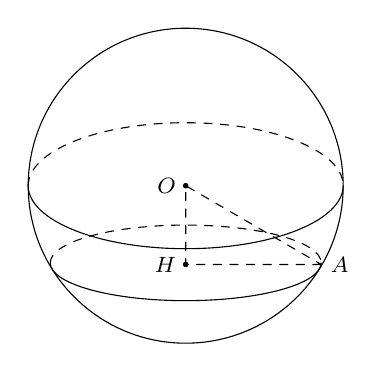
\begin{tikzpicture}[scale=0.8, font=\footnotesize, line join=round, line cap=round, >=stealth]
				\def \r{2.5}
				\def \a{0.86*\r}
				\def \b{0.5*\r}
				\def \c{0.49*\r}
				\coordinate (o) at (0,0);
				\draw [] (o) circle (\r);
				\coordinate (m) at (0,\r);     % Định tọa độ điểm B
				\coordinate (n) at (0,-\r);
				\coordinate (p) at (0,-\b);
				\draw [] (-\r,0) arc [start angle= 180, end angle= 360, x radius=\r, y radius=1];
				\draw [dashed] (-\r,0) arc [start angle= 180, end angle= 0, x radius=\r, y radius=1];
				\draw [] (-\a,-\c) arc [start angle= 180, end angle= 360, x radius=\a, y radius=.6];
				\draw [dashed] (-\a,-\c) arc [start angle= 180, end angle= 0, x radius=\a, y radius=.6];
				\draw[dashed] (\a,-\b)node[right]{$A$} --(p)--(o)--cycle;
				\draw (o) node[left] {$O$};
				%\draw (m) node[above] {$M$};
				%\draw (n) node[below] {$M'$};
				\draw (p) node[left] {$H$};
				\draw[fill] (o) circle [radius=1pt];
				%\draw[fill] (m) circle [radius=1pt];
				%\draw[fill] (n) circle [radius=1pt];
				\draw[fill] (p) circle [radius=1pt];
		\end{tikzpicture}}
	}
\end{ex}

%%==========Câu 37
\begin{ex}%[2H3Y1-1]%
	Trong không gian $ Oxyz  $, cho điểm $ M(1;-2;-3) $. Hình chiếu vuông góc của điểm $ M $ lên mặt phẳng $ (Oyz) $ là
	\choice
	{\True $ Q(0;-2;-3) $}
	{$ K(1;0;3) $}
	{$ P(1;0;-3) $}
	{$ N(1;-2;0) $}
	\loigiai{
		Tọa độ hình chiếu vuông góc của điểm $ M $ lên mặt phẳng $ (Oyz) $ là $ (0;-2;-3) $.
	}
\end{ex}

%%==========Câu 38
\begin{ex}%[2H3Y1-1]
	Trong không gian $Oxyz$, Cho hai điểm $A(1;1;-1)$ và $B(2;3;2)$. Véctơ $\vec{AB}$ có tọa độ
	\choice
	{\True $(1;2;3)$}
	{$(-1;-2;3)$}
	{$(3;5;1)$}
	{$(3;4;1)$}
	\loigiai{
		$\vec{AB}=(2-1;3-1;2+1)=(1;2;3)$
	}
	%<MyLT>
\end{ex}


%%==========Câu 39
\begin{ex}%[2H3Y2-2]
	Trong không gian $Oxyz$, cho mặt phẳng $(P)\colon x+y-z+2=0$. Một véc-tơ pháp tuyến của mặt phẳng $(P)$ có tọa độ là
	\choice
	{$(2;1;1)$}
	{$(1;2;1)$}
	{\True $(1;1;-1)$}
	{$(1;-2;1)$}
	\loigiai{
		Một véc-tơ pháp tuyến của $(P)$ là $\overrightarrow{n}=(1;1;-1)$.
	}
	%<MyLT>
\end{ex}


%%==========Câu 40
\begin{ex}%[2H3Y3-1]
	Trong không gian $Oxyz$, cho đường thẳng $d\colon \dfrac{x}{2}=\dfrac{y}{1}=\dfrac{z-1}{2}$. Một véc-tơ chỉ phương của $d$ là
	\choice
	{$\vec{u}=(0;0;1)$}
	{$\vec{u}=(0;0;-1)$}
	{$\vec{u}=(2;6;2)$}
	{\True $\vec{u}=(2;1;2)$}
	\loigiai{
		Ta có véc-tơ chỉ phương của $d$ là $\vec{u}=(2;1;2)$.
	}
\end{ex}


%%==========Câu 41
\begin{ex}%[2H3B1-1]
	Trong không gian $Oxyz$, cho hai điểm $A(2;1;1)$, $B(0;2;3)$. Tìm tọa độ điểm $M$ sao cho $\overrightarrow{AM}=\dfrac{2}{3}\overrightarrow{AB}$.
	\choice
	{$M\left(-\dfrac{4}{3};\dfrac{2}{3};\dfrac{4}{3}\right)$}
	{$M\left(1;\dfrac{3}{2};1\right)$}
	{\True $M\left(\dfrac{2}{3};\dfrac{5}{3};\dfrac{7}{3}\right)$}
	{$M\left(2;3;4\right)$}
	\loigiai{
		Gọi $M(x;y)$, theo bài ra ta có
		\begin{align*}
			&\, \overrightarrow{AM}=\dfrac{2}{3}\overrightarrow{AB}\Leftrightarrow 3\overrightarrow{AM}=2\overrightarrow{AB}\\
			\Leftrightarrow &\, 3(x-2;y-1;z-1)=2(-2;1;2)\\
			\Leftrightarrow &\,\heva{&3x-6=-4\\ &3y-3=2\\ &3z-3=4}\Leftrightarrow\heva{&x=\dfrac{2}{3}\\ &y=\dfrac{5}{3}\\ &z=\dfrac{7}{3}}
		\end{align*}
	}
\end{ex}


%%==========Câu 42
\begin{ex}%[2H3B1-3]
	Trong không gian $ Oxyz $, biết phương trình mặt cầu $(S):x^2+y^2+z^2=25 $ cắt mặt phẳng $(P): x+y+z=3\sqrt{3}$ theo giao tuyến là một đường tròn có bán kính $ r $. Khi đó giá trị của $ r $ là
	\choice
	{$5$}
	{$3$}
	{$\tfrac{5}{3}$}
	{\True $4$}
	\loigiai{
		Mặt cầu $(S):x^2+y^2+z^2=25 $ có tâm $ O(0; 0; 0)$ và bán kính $ R=5 $.\\
		Ta có $\mathrm{d}=\mathrm{d}\left(O, (P)\right)=\dfrac{|0+0+0-3\sqrt{3}|}{\sqrt{1^2+1^2+1^2}}=3. $\\
		Suy ra bán kính đường tròn giao tuyến là
		$ r=\sqrt{R^2-\mathrm{d}^2}=\sqrt{5^2-3^2}=4 $.
	}
	%<MyLT>
\end{ex}


%%==========Câu 43
\begin{ex}%[2H3K2-6]
	Trong không gian $Oxyz$, cho ba điểm $A(1;1;3)$, $B(-1;3;2)$, $C(-1;2;3)$. Khoảng cách từ gốc tọa độ đến mặt phẳng $(ABC)$ bằng
	\choice
	{$\dfrac{3}{2}$}
	{\True $3$}
	{$\sqrt{3}$}
	{$\dfrac{\sqrt{3}}{2}$}
	\loigiai{
		Ta có $\vec{AB}=(-2;2;-1)$ và $\vec{AC}=(-2;1;0)$ nên mặt phẳng $(ABC)$ nhận $\vec{n}=[\vec{AB},\vec{AC}]=(1;2;2)$ là véc-tơ pháp tuyến.\\
		Phương trình mặt phẳng $(ABC)$ là $(x-1)+2(y-1)+2(z-3)$ hay $x+2y+2z-9=0$.\\
		Khi đó $\mathrm{d}\left(O,(ABC)\right)=\dfrac{|-9|}{\sqrt{1^2+2^2+2^2}}=3$.
	}
\end{ex}

%%==========Câu 44
\begin{ex}%[2H3B3-2]
	Trong không gian $Oxyz$, cho hai điểm $A(-1;2;2)$, $B(3;-2;-4)$. Khi đó mặt phẳng trung trực của đoạn thẳng $AB$ có phương trình là
	\choice
	{\True $2x-2y-3z-5=0$}
	{$2x-2y-3z=0$}
	{$2x+2y-3z-5=0$}
	{$2x-2y+3z+1=0$}
	\loigiai{
		Ta có $\overrightarrow{AB}=(4;-4;-6)$ cùng phương với $\overrightarrow{n}=(2;-2;-3)$. \\
		Mặt phẳng trung trực của $AB$ đi qua trung điểm $I(1;0;-1)$ của $AB$ và có véc-tơ pháp tuyến $\overrightarrow{n}=(2;-2;-3)$.\\
		Vậy phương trình mặt phẳng trung trực của $AB \colon 2x-2y-3z-5=0$. }
\end{ex}

%%==========Câu 45
\begin{ex}%[1D3Y3-3]
	Cho cấp số cộng $ (u_n) $ có số hạng đầu $ u_1 =2$, số hạng thứ ba $ u_3=8 $. Giá trị công sai bằng
	\choice
	{$ 10 $}
	{\True $ 3 $}
	{$ 5 $}
	{$ 4 $}
	\loigiai{
		Gọi $ d $ là công sai của cấp số cộng, suy ra $ u_3=u_1+2d \Leftrightarrow d=\dfrac{u_3-u_1}{2}=\dfrac{8-2}{2}=3$.}
\end{ex}


%%==========Câu 46
\begin{ex}%[1D4Y1-3]
	$\lim\dfrac{1-n}{1-3n^2}$ bằng
	\choice
	{\True $0$}
	{$\dfrac{1}{3}$}
	{$1$}
	{$-\dfrac{1}{3}$}
	\loigiai{
		Ta có $\lim\dfrac{1-n}{1-3n^2}=\lim\dfrac{\dfrac{1}{n^2}-\dfrac{1}{n}}{\dfrac{1}{n^2}-3}=0$.
	}
\end{ex}

%%==========Câu 47
\begin{ex}%[1D2B2-1]
	Với $k,n$ là hai số tự nhiên tùy ý thỏa mãn $k\le n$, mệnh đề nào dưới đây đúng?
	\choice
	{ $\mathrm{A}_n^k=\dfrac{k!\cdot (n-k)!}{n!}$}
	{\True $\mathrm{A}_n^k=\dfrac{n!}{(n-k)!}$}
	{  $\mathrm{A}_n^k=\dfrac{n!}{k!}$}
	{ $\mathrm{A}_n^k=\dfrac{n!}{k! \cdot (n-k)!}$}
	\loigiai{
		Áp dụng công thức tính số chỉnh hợp chập $k$ của $n$ phần tử, ta có $\mathrm{A}_n^k=\dfrac{n!}{(n-k)!}$. }
	%<MyLT>
\end{ex}

%%==========Câu 48
\begin{ex}%[1D2B5-2]
	Một đội gồm $5$ nam và $8$ nữ. Lập một nhóm gồm $4$ người hát tốp ca, tính xác suất để trong $4$ người được chọn có ít nhất $3$ nữ.
	\choice
	{$\dfrac{73}{143}$}
	{$\dfrac{56}{143}$}
	{\True $\dfrac{70}{143}$}
	{$\dfrac{87}{143}$}
	\loigiai{
		Không gian mẫu là chọn tùy ý $4$ người từ $13$ người.\\
		Suy ra số phần tử của không gian mẫu là $\left| \Omega \right|=\mathrm{C}_{13}^4=715$.\\
		Gọi $A$ là biến cố ``4 người được chọn có ít nhất 3 nữ''. Ta có hai trường hợp thuận lợi cho biến cố $A$ như sau:\\
		\begin{itemize}
			\item \textbf{TH1:} Chọn $3$ nữ và $1$ nam, có $\mathrm{C}_8^3\mathrm{C}_5^1$ cách.
			\item \textbf{TH2:} Chọn cả $4$ nữ, có $\mathrm{C}_8^4$ cách.
		\end{itemize}
		Suy ra số phần tử của biến cố $A$ là $\left| {\Omega}_A\right|=\mathrm{C}_8^3\mathrm{C}_5^1+\mathrm{C}_8^4=350$.\\
		Vậy xác suất cần tính $\mathrm{P}(A)=\dfrac{\left| {\Omega}_A\right|}{\left| \Omega \right|}=\dfrac{350}{715}=\dfrac{70}{143}$.
	}
	
\end{ex}

%%==========Câu 49
\begin{ex}%[1H3Y2-3]
	\immini[thm]{Cho hình lập phương $ABCD.A'B'C'D'$. Góc giữa hai đường thẳng $BA'$ và $B'C'$ bằng
		\choice
		{$45^\circ$}
		{$30^\circ$}
		{$60^\circ$}
		{\True $90^\circ$}}{
		\begin{tikzpicture}[line cap=round,line join=round,font=\footnotesize,>=stealth,scale=0.8]
			\fill (0,0) coordinate [label=left:$A$] (A) circle(1pt)
			(4,0) coordinate [label=below right:$B$] (B) circle(1pt)
			(40:2) coordinate [label=left:$D$] (D) circle(1pt)
			(90:3) coordinate [label=left:$A'$] (A') circle(1pt)
			($(B)+(D)$) coordinate [label=right:$C$] (C) circle(1pt)
			($(A')+(B)$) coordinate [label=right:$B'$] (B') circle(1pt)
			($(A')+(C)$) coordinate [label=right:$C'$] (C') circle(1pt)
			($(A')+(D)$) coordinate [label=above:$D'$] (D') circle(1pt);
			\draw (C')--(B')--(A')--(A)--(B)--(C)--(C')--(D')--(A')--(B)--(B');
			\draw [dashed] (A)--(D)--(D') (D)--(C);
	\end{tikzpicture}}
	\loigiai{
		Vì $B'C' \perp (ABB'C')$ nên $B'C' \perp BA'$
	}
\end{ex}

%%==========Câu 50
\begin{ex}%[1H3K4-3]
	Cho hình chóp $S.ABCD$ có đáy $ABCD$ là hình vuông, $SA$ vuông góc với mặt đáy. 
	\begin{center}
		\begin{tikzpicture}[scale=0.7, line join=round, line cap=round]
			\tikzset{label style/.style={font=\footnotesize}}
			\tkzDefPoints{0/0/A,-1.3/-1.6/B,2.5/-1.6/C}
			\coordinate (D) at ($(A)+(C)-(B)$);
			\coordinate (S) at ($(A)+(0,3)$);
			\tkzDrawPolygon(S,B,C,D)
			\tkzDrawSegments(S,C)
			\tkzDrawSegments[dashed](A,S A,B A,D)
			\tkzDrawPoints[fill=black,size=4](D,C,A,B,S)
			\tkzLabelPoints[above](S)
			\tkzLabelPoints[below](A,B,C)
			\tkzLabelPoints[right](D)
		\end{tikzpicture}
	\end{center}
	Góc giữa hai mặt phẳng $(SCD)$ và $(ABCD)$ bằng
	\choice
	{$\widehat{ASD}$}
	{$\widehat{SCA}$}
	{$\widehat{SCB}$}
	{\True $\widehat{SDA}$}
	\loigiai{
		Ta có: $\heva{&CD\perp AD\\&CD\perp SA}$ nên $CD\perp (SAD)$ $\Rightarrow CD\perp SD$ nên góc của $(SCD)$ và $(ABCD)$ bằng $\widehat{SDA}$.
	}
\end{ex}
\Closesolutionfile{ans}
\indapan{10}{ans/ansVN-1}

%====================
